\section{Ziel}
    In diesem Versuch sollen die Topologien verschiedener Strukturen im Micrometerbereich sowie die von Speicherdiscs wie CD, DVD und Blu-Ray untersucht werden. Dazu wird die Methode der \textit{atomic force
    microscopy} (AFM) verwendet, die auf der Auslenkung einer wenigen Nanometer großen Spitze aufgrund der Wechselwirkung zwischen dieser und den Oberflächenatomen basiert. Da diese Wechselwirkungen nicht
    auf Elektrostatik basieren, können im Vergleich zum Rastertunnelmikroskop auch nicht leitende Proben vermessen werden.    
    
\section{Theoretische Grundlagen}
    \subsection{Messprinzip}
        Das klassische Messprinzip der AFM ist in Abbildung \ref{fig:prinzip} visualisiert. Eine \textbf{Messspitze} (\textit{Probe Tip}), die an einem \textbf{Cantilever} befestigt ist, wird auf eine 
        Entfernung von wenigen Angström bis einigen \SI{100}{\nano\metre} an die Probenoberfläche gebracht. Die zwischen der Messspitze und den Oberflächenatomen wirkende Kraft resultiert aus verschiedenen
        distanzabhängigen \textbf{Wechselwirkungen} und wird auf den Cantilever übertragen. Verschiedene \textbf{Detektionssysteme} erlauben es die wirkende Kraft über den Cantilever zu messen und so den 
        Abstand zwischen Messspitze und Oberfläche zu bestimmen. In Kombination eines elektronischen Feedback-Loops mit \textbf{Piezoelementen}, die die Probe relativ zur Messspitze in x-, y- und z-Richtung
        verschieben können, ist es möglich diese Abstandsmessung auf der gesamten Probe durchzuführen und so ein Höhenprofil der Oberfläche zu ermitteln. Da je nach Distanz verschiedene Kräfte dominieren und
        der Feedback-Loop es auch ermöglicht auf verschiedene Weise über die Probe zu rastern, kann die AFM in mehreren \textbf{Messmodi} betrieben werden.

        \FloatBarrier

        \begin{figure}[h]
          \centering
          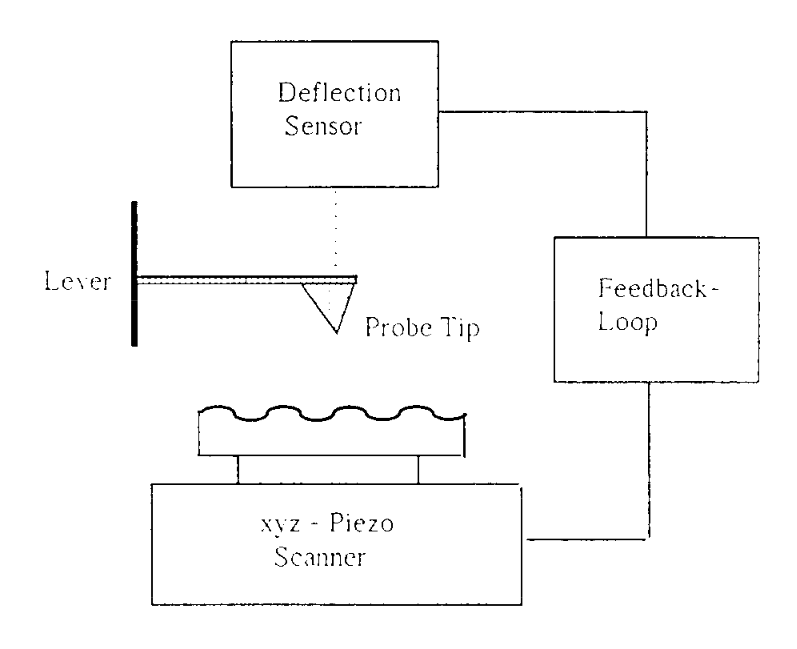
\includegraphics[width = 0.4\textwidth]{pictures/prinzip.png}
          \caption{Schematische Abbildung eines Atomic-Force Mikroskops bestehend aus Spitze und Cantilever, Feedback-Loop, Auslenkungssensor und Piezoelementen. Entnommen aus \cite{meyer_atomic_1992}}
          \label{fig:prinzip}
        \end{figure}
    
        \FloatBarrier


      \subsection{Wechselwirkungen}

        \subsubsection{Spitze - Oberfläche}

          \FloatBarrier

          \begin{wrapfigure}[38]{L}{8.2cm}
            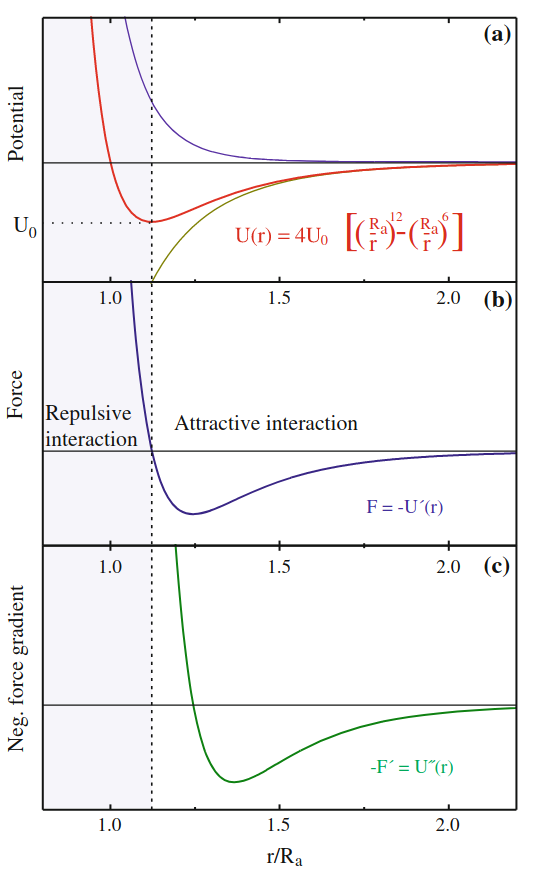
\includegraphics[scale = 0.42]{pictures/LJ.png}
            \caption{Zusammensetzung des gesamten Potentials zwischen Messspitze und Oberfläche aus anziehendem und abstoßendem Potential in der Beschreibung eines Lennard-Jones-Potentials. Entnommen aus \cite{voigtlander_scanning_2015}}
            \label{fig:LJ}
          \end{wrapfigure}
          \FloatBarrier

          Zur Vermessung des Höhenprofils der Oberfläche wird die distanzabhängige Kraft zwischen Messspitze und Oberfläche genutzt. Das zugehörige Potential wird als Lennard-Jones-Potential 

          \begin{equation*}
            \text{U(R)} = 4\text{U}_0 \left[ \left(\frac{\text{R}_{\text{a}}}{\text{r}}\right)^{12} - \left(\frac{\text{R}_{\text{a}}}{\text{r}}\right)^{6} \right]
          \end{equation*}

          angenähert, das einen positiven und demnach repulsiven Anteil und einen attraktiven Anteil besitzt, und in Abbildung \ref{fig:LJ} (a) mitsamt der resultierenden Kraft (b) und dem zugehörigen
          Kraftgradienten (c) dargestellt ist.


          

          Das Potential setzt sich aus verschiedenen Wechselwirkungen zusammen, die für unterschiedliche Entfernungen dominant sind.\newline 
          Der attraktive Bereich für Abstände über \SI{1}{\nano\metre} resultiert hauptsächlich aus den \textit{Van-der-Waals-Kräften}. Diese beschreiben die Anziehung zweier eigentlich neutraler Atome durch die 
          spontane Entstehung von fluktuierenden Dipolen. Entsteht in einem Atom eine 
          spontaner Dipol, wird im benachbarten Atom ebenfalls ein Dipol induziert und die Atome ziehen sich an. Das zugehörige Potential fällt mit $\frac{1}{\text{r}^6}$ ab und ist demnach langreichweitig. 
          Deswegen wechselwirkt nicht nur das vorderste Atom der Spitze mit der Oberfläche, sondern auch dahinterliegende.\newline

          Für Distanzen unter \SI{1}{\nano\metre} kommt es zu chemischen Bindungen, bei denen die Orbitale der beteiligten Atome hybridisieren. Führt dies zu einer Verringerrung der Gesamtenergie wirken diese 
          Bindungen attraktiv. Erhöht sich die Gesamtenergie wirken die Bindungen repulsiv.

          Relevanter für diese Distanzen unter \SI{1}{\angstrom} ist das Auftreten stark repulsiver Wechselwirkungen. Die dominante Abstoßung folgt aus dem Pauli-Prinzip, nach dem zwei Elektronen mit dem 
          selben Spin nicht den selben Zustand besetzen dürfen. Bei sehr geringen Distanzen führt der Überlapp der Orbitale dazu, dass Elektronen in höhere unbesetzte Bänder ausweichen müssen. Dies führt zu einer 
          starken Erhöhung der Gesamtenergie und somit zu einer repulsiven Kraft. Zusätzlich kann auch Coulombabstoßung zwischen den Kernen auftreten, wenn diese nicht komplett durch ihre Elektronen 
          abgeschirmt sind.

          Falls zwischen der Spitze und der Oberfläche eine Potentialdifferenz vorliegt, kommt es zusätzlich zu elektrostatischen Kräften. Diese können jedoch vermieden werden, indem die Potentialdifferenz durch
          das Anlegen einer entsprechenden Spannung kompensiert wird.\newline

          Da die entstehenden Kräfte in Bereich einiger Nanonewton liegen und die Auslenkungen des Systems demenstprechend sehr gering sind, ist die Messung der Auslenkung besonders anfällig für externe Erschütterungen des Mikroskops.
          
        \newpage
        \subsubsection{Cantilever - Spitze - Oberfläche}

          \FloatBarrier

          \begin{wrapfigure}[35]{L}{8cm}
            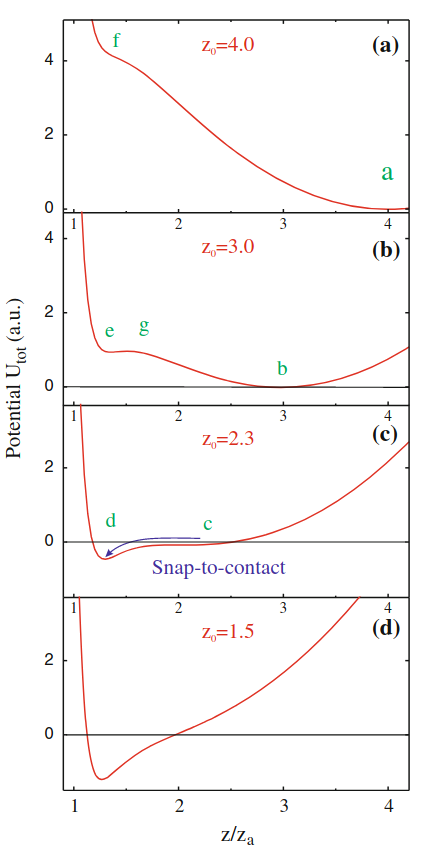
\includegraphics[scale = 0.45]{pictures/pot_contact.png}
            \caption{Mit abnehmender Distanz zwischen Messspitze und Probe entsteht zunächst ein zweites lokales Minimum nahe der Oberfläche. Ab einem gewissen Abstand verschwindet das erste lokale Minima und die Messspitze springt an die Oberfläche (snap-to-contact). Entnommen aus \cite{voigtlander_scanning_2015}}
            \label{fig:pot_contact}
          \end{wrapfigure}

          \FloatBarrier      
          %
          In einem AFM-Aufbau ist die Spitze an einem Cantilever befestigt, der als Feder fungiert und so ebenfalls Einfluss auf die Gesamtkraft nimmt. Nach dem Hook'schen Gesetz ergibt sich ein Potential 
          %
          \begin{equation*}
            \text{U}_{\text{F}} = \frac{1}{2} \text{k} \left(\text{z} - \text{z}_0\right)^2 \, ,
          \end{equation*}
          %
          das quadratisch in der Auslenkung z um eine Ruheposition z$_0$ und proportional zur Federkonstante k ist. 
          Die Auswirkungen dieses Potentials lassen sich über Abbildung \ref{fig:pot_contact} erklären, in der 
          das Potential, für verschiedene Ruhepositionen auf das Lennard-Jones-Potential addiert, dargestellt ist. Wenn der Cantilever weit von der Oberfläche entfernt ist (a), besitzt das Potential ein 
          Minimum an der Ruheposition des Cantilevers. Wird der Cantilever mitsamt der Spitze angenähert (b), entsteht ein zweites lokales Minimum. Dieses liegt nah an der Oberfläche und ist von der Ruheposition
          nicht zu erreichen, da ein Maximum die beiden Minima trennt. Ab einer Grenze geht dieses Maximum in einen Sattelpunkt über und ein Übergang in das zweite Minimum wird möglich. Dieser Übergang wird als
          snap-to-contact bezeichnet und beschreibt einen Endzustand, in dem die abstoßenden Kräfte ein weiteres Annähern an die Probe verhindern. 




        \newpage
        \subsubsection{Kraft-Distanz-Kurven}

          Aus den gegebenen Potentialverläufen lässt sich begründen, welche Kraft auf das System aus Messspitze und Cantilever wirkt, wenn es an die Oberfläche herangebracht oder entfernt wird. Dieses Verhalten
          wird in Kraft-Distanz-Kurven dargestellt, die die Kraft für einen vollen Zyklus aus Annäherung und Entfernung gegen den Abstand auftragen. Zum Verständnis der folgenden Beschreibung werden die Punkte A) bis E) in Abbildung \ref{fig:forcedist} beschrieben. Charakteristisch für den Annäherungsprozess ist zunächst
          eine Kräftefreiheit A), bis zu einem plötzlichem negativem Kraftgradienten B), der einer Anziehung zur Probe entspricht und aufgrund des snap-to-contacts auftritt. Dabei wirken die attraktive Van-der-Waals-Kraft und für eine Messung außerhalb des Vakuums Kapillarkräfte. Da mit dem snap-to-contact die Messspitze auf 
          der Oberfläche aufliegt, steigt die Kraft bei weiterer Annäherung aufgrund der repulsiven Pauli-Kraft linear C) bis zu einem Maximum, bei dem das Annähern gestoppt wird. Wenn das Messsystem entfernt wird, sinkt die Kraft analog zu ihrem 
          vorherigen Anstieg D), bis die wirkende Kraft bei dem selben Abstand wieder ihr Vorzeichen wechselt. In Abhängigkeit von der Stärke der attraktiven Adhesionskräfte verbleibt die Spitze nun länger in Kontakt E) und es treten stärker anziehende Kräfte als beim snap-to-contact auf. 
          
          \FloatBarrier

          \begin{figure}[h]
            \centering
            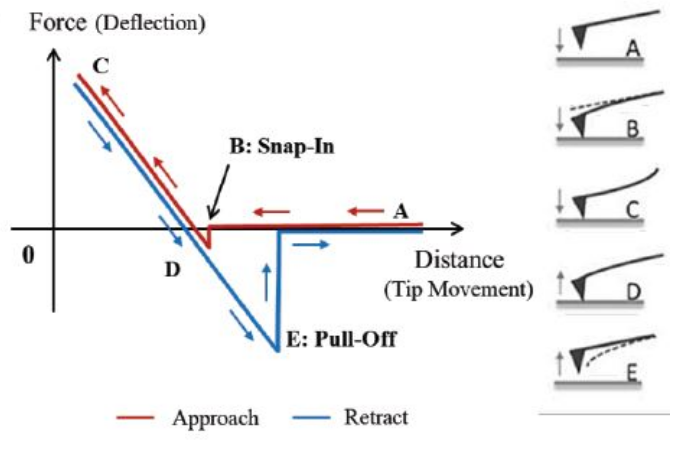
\includegraphics[width = 0.4\textwidth]{pictures/forcedist.png}
            \caption{Eine vollständige Kraft-Distanz-Kurve mit den entsprechenden Positionen und Auslenkung der Cantilever an ausgewählten Punkten a) bis f). Entnommen aus \cite{park_systems_force-distance_nodate}}
            \label{fig:forcedist}
          \end{figure}
        
          \FloatBarrier
          
          Der lineare Anstieg und Abfall der Kurve hängt dabei von der Härte der Probe ab. Da die Messspitze nur schlecht in besonders harte Proben eindringen kann, steigt die Kraft, wie in Abbildung \ref{fig:force_hard_soft} zu sehen, stärker an und sinkt auch schneller ab. Die Messspitze löst sich
          bei gleicher Kraft von der Oberfläche, wie bei einer weichen Probe, erreicht diese aber bereits bei geringerem Abstand. Mit einer höheren Federkonstante des Cantilevers kann der Scanbereich der
          Kraft-Distanz-Kurve auf Kosten der Kraftauflösung erweitert werden, da der Cantilever größere Kräfte aushält, bevor er inelastisch verformt wird.





          \begin{figure}[h]
            \centering
            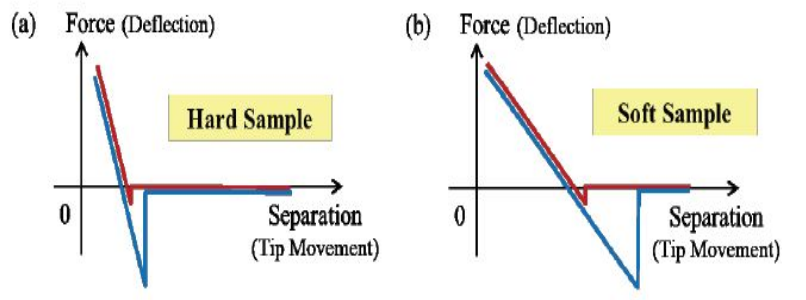
\includegraphics[width = 0.4\textwidth]{pictures/force_hard_soft.png}
            \caption{Die Kraft-Distanz-Kurve einer harten a) und einer weichen Probe b) zeigen die unterschiedlich starken Steigungen der Kraftkurve. Entnommen aus \cite{park_systems_force-distance_nodate}}
            \label{fig:force_hard_soft}
          \end{figure}


          \FloatBarrier






      \newpage


      \subsection{Messspitze und Cantilever}
        Die Messspitze und der Cantilever gehören zu den Hauptbauteilen, da auf sie die Kraft wirkt beziehungsweise sie die Kraft weitergeben, die später Rückschlüsse auf die Topologie der Oberfläche geben soll.
        Deswegen müssen sie spezielle Eigenschaften besitzen, die in der Anwendung auch unterschiedliche Messmodi ermöglichen können.

        \subsubsection*{Messspitze}
          Die Messspitze ist das Bauteil, das der Oberfläche am nähesten kommt und tatsächlich mit ihr wechselwirkt. Eine unendliche glatte Oberfläche könnte mit einer stumpfen Spitze vermessen werden. Wenn
          die Oberfläche jedoch nicht glatt ist und distinkte Hindernisse gemessen werden sollen, kommen neue Anforderungen auf die am besten über die in Abbildung \ref{fig:defekte} abgebildeten Messdefekte
          zu begründen sind. In Abbildung \ref{fig:defekte} a) und b) ist zu erkennen, dass eine zu stumpfe Spitze womöglich nicht in der Lage ist zu steile Objekte zu erkennen. Das gemessene Profil (rot) ist
          immer eine Faltung aus dem Profil der Spitze und dem der Oberfläche. Um nun kleine und steile Signale zu detektieren, muss die Spitze steiler zusammenlaufen als der steilste Gradient an der 
          Probenoberfläche und dünner sein, als das kleinste Objekt. In der Anwendung sind Spitzendurchmesser im einstelligen Micrometerbereich und Krümmugsradien von wenigen Nanometern möglich. Eine weitere
          Quelle für Defekte sind die in Abbildung \ref{fig:defekte} zu sehenden Beulen an der sonst flachen Spitze. Diese müssen unbedingt vermieden werden, da sie nicht vorhandene Strukturen an der Oberfläche
          im Höhenprofil erzeugen. 
        
          \FloatBarrier

          \begin{figure}[h]
            \centering
            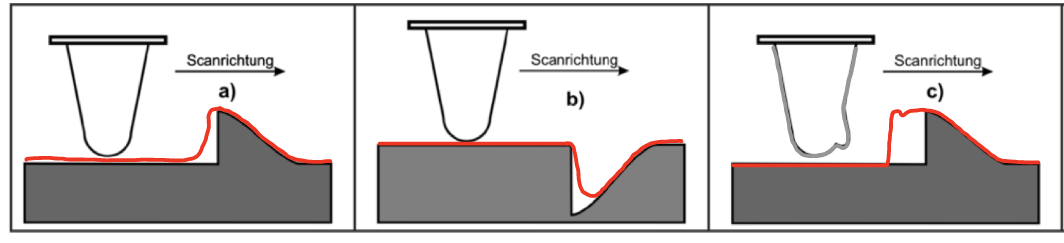
\includegraphics[width = 0.8\textwidth]{pictures/defekte.png}
            \caption{Es können Messartifakte auftreten, wenn die Spitze nicht in der Lage ist steile An- oder Abstiege im Höhenprofil zu erkennen oder Defekte an der Messspitze vorhanden sind. Bearbeitet aus \cite{tu_dortmund_versuchsanleitung_nodate}}
            \label{fig:defekte}
          \end{figure}
        
          \FloatBarrier

        
          \newpage
        \subsubsection*{Cantilever}
          Der Cantilever nimmt die auf die Messspitze wirkende Kraft auf, indem er sich verbiegt. Um diese Verbiegung zu Kraftmessung gut detektieren zu können, muss auch der Cantilever bestimmte Eigenschaften
          besitzen. Diese sind besonders an verschiedene Messmodi gekoppelt. Da der Cantilever sehr geringe Kräfte im Bereich von $10^{-9} \si{\newton}$ detektierbar machen muss, soll er sich bereits bei diesen
          Kräften genügend auslenken. Hier werden Federkonstanten von ca. $10 \si{\newton\per\metre}$, die detektierbare Auslenkungen im Angström Bereich erlauben. Zusätzlich soll der Cantilever eine  
          Resonanzfrequenz >> $10 \si{\kilo\hertz}$ besitzen, um in dynamischen Messungen, bei denen sich der Cantilever bewegt, die Messgeschwindigkeit zu erhöhen. Aufgrund der geringen Federkonstante folgt
          aus der Anforderung an die Resonanzfrequenz

          \begin{equation*}
            \omega_{\text{Res}} = \sqrt{\frac{\text{k}}{\text{m}}}
          \end{equation*}

          eine sehr geringe Masse des Cantilevers im Microgrammbereich.


          \begin{figure}[h]
            \centering
            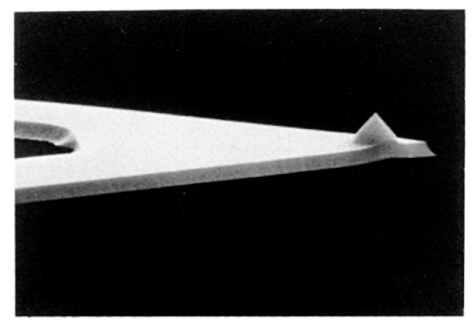
\includegraphics[width = 0.6\textwidth]{pictures/Cantilever_Spitze.png}
            \caption{Teil eines Cantilevers mit angebrachter Spitze, die einen maximalen Durchmesser von circa $5 \si{\micro\metre}$ besitzt. Entnommen aus \cite{wiesendanger_scanning_1998}}
            \label{fig:Cantilever_Spitze}
          \end{figure}
        
          \FloatBarrier




      \newpage
      \subsection{Detektionssysteme}
          Zur Bestimmung der wirkenden Kraft muss in statischen Messung die Auslenkung des Cantilevers und in dynamischen Messungen dessen Schwingungsamplitude gemessen werden. Dafür kann auf elektrische
          oder optische Detektionsmechanismen zurückgegriffen werden. 
          Zu den elektrischen Detektionsmechanismen gehören die Kondensatormethode, die Elektronentunnelmethode sowie Piezoelektrische Methoden. Bei der Kondensatormethode bilden der Cantilever und eine
          Elektrode einen Kondensator, dessen abstandsabhängige Kapazität gemessen wird. Während diese Methode sehr stabil und einfach zu betreiben ist, stellt die elektronstatische Anziehung des Cantilevers
          an die Elektrode ein Problem dar. Bei der atomar auflösenden Elektronentunnelmethode wird der Tunnelstrom zwischen einer Spitze eines Elektronentunnelmikroskops (STM) und dem Cantilever gemessen. 
          Der Betrieb im Vakuum ist jedoch umständlich und die Wechselwirkung der STM Spitze mit dem Cantilever beeinflusst die genaue Distanzmessung. Bei den piezoelektrischen Methoden induziert die Verbiegung
          des Cantilevers eine Spannung in piezoelektrischen Kristallen, die direkt oder über eine Widerstandsänderung gemessen werden und so zur Distanzberechnung genutzt werden kann. 
          Besonders sensitive Messungen lassen sich mit einer optischen Interferometriemessung durchführen, bei der durch Auslenkung des Cantilevers die optische Weglänge des Lichts geändert und aus dem so
          veränderten Interfernzeffekten eben diese Auslenkung berechnet wird.

          Ein weitere, technisch deutlich einfacher umsetzbare Technik beruht auf dem Lichtzeigerprinzip. Hier wird ein Laserstrahl auf den Cantilever geschossen und von diesem auf eine Viersegmentdiode 
          reflektiert. Diese besteht aus vier einzelnen Dioden und kann aus dem Intensitätsverhältnis der einzelnen Dioden die Position des Laserstrahls relativ zum Zentrum der Photdiode bestimmen. Aufgrund
          des Einsatzes von vier Photdioden lässt sich so neben der vertikalen auch die laterale Auslenkung bestimmen. Die mit dieser Methode minimal messbare vertikale Auslenkung ist unter anderem proportional
          zur Wellenlänge des Lasers und der Spotgröße des Laserstrahl auf dem Cantilevers, da beides den störenden Einfluss der Interferenz senkt. Durch Optimierung dieser Parameter lassen sich mit dem
          Lichtzeigerprinzip vertikale Auslenkung ab einem Bereich um circa $1 \si{\micro\metre}$ messen.


          \FloatBarrier

          \begin{figure}[h]
            \centering
            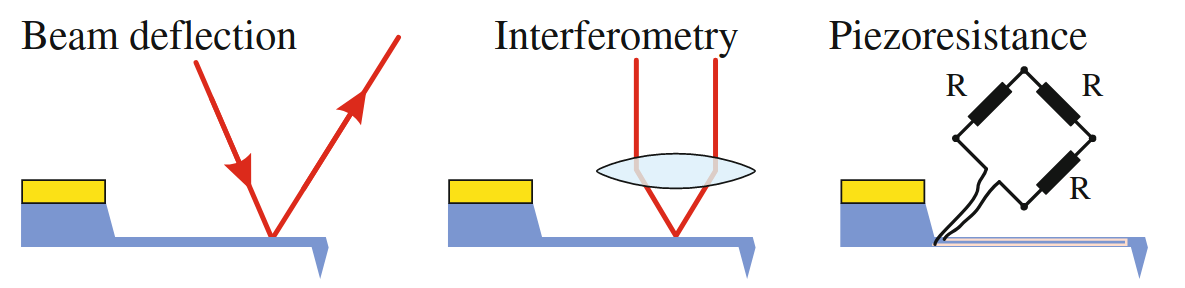
\includegraphics[width = 0.4\textwidth]{pictures/detektion.png}
            \caption{Schematische Darstellung der Auslenkungsdetektion (v.l.) über das Lichtzeigerprinzip, die Interferometriemessung und der piezoelektrischen Messung. Entnommen aus \cite{park_systems_force-distance_nodate}}
            \label{fig:detektion}
          \end{figure}
        
          \FloatBarrier

      

      \newpage
      \subsection{Messmodi}
          In der AFM können verschiedene Messmodi genutzt werden, um unterschiedliche Eigenschaften der Oberfläche oder auch allgemeiner unterschiedliche Oberfläche zu untersuchen. Grundlegend wird dabei 
          zwischen statischen und dynamischen Messungen sowie Messungen mit oder ohne Kontakt zur Oberfläche unterschieden. 

          Wenn die Messspitze in Kontakt zur Oberfläche steht, liegt der Abstand zwischen Messspitze und Oberfläche im repulsiven Bereich des Potentials unter \SI{10}{\nano\metre} und die Messspitze wird von 
          der Oberfläche weggedrückt. In diesem Modus lässt sich die Topologie der Oberfläche beinahe atomar auflösen. Ein zusätzlicher Vorteil dieses Modus ist, dass die Messspitze durch flüssige 
          Oberflächenkontaminationen hindurchmisst. Der konstante Kontakt zur Oberfläche birgt die Gefahr des Abbrechens der Messspitze oder Beschädigung der Oberfläche. Messung im \textit{contact mode}
          können statisch und dynamisch durchgeführt werden. In statischen Messungen wird der Cantilever durch die wirkende Kraft verbogen und diese Biegung gemessen. Es kann entweder die Höhe der Messspitze
          über der Oberfläche konstant gehalten und die Änderung der Biegung gemessen werden (\textit{constant height}) oder die Biegung  und demenstprechend auch die Kraft konstant gehalten werden, indem
          der Abstand zwischen Messspitze und Oberfläche durchgehend nachreguliert wird (\textit{constant force}). Diese beiden Methoden sind in Abbildung \ref{fig:modi} dargestellt. 
          
          \FloatBarrier

          \begin{figure}[h]
            \centering
            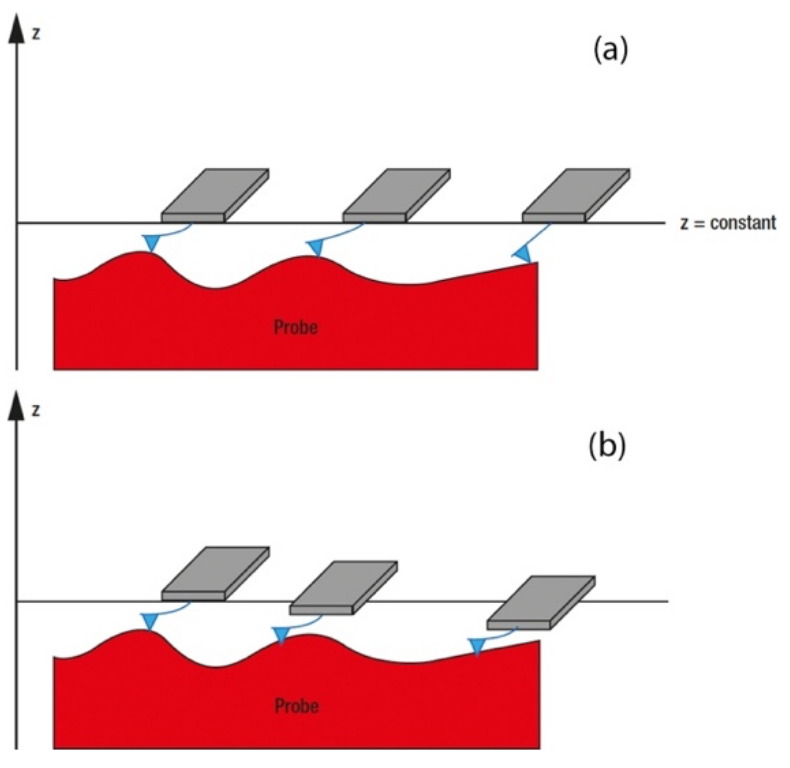
\includegraphics[width = 0.4\textwidth]{pictures/const_height_force.png}
            \caption{In Ausschnitt a) ist das Rastern bei konstanter Entfernung z zur Probenoberfläche und in Ausschnitt b) beim Erhalten einer konstanten Kraft auf die Spitze dargestellt. Entnommen aus \cite{voigtlander_scanning_2015}}
            \label{fig:modi}
          \end{figure}
        
          \FloatBarrier  
          \newpage
                 
          In dynamischen Messungen schwingt das System aus Cantilever und Messspitze mit dessen 
          Resonanzfrequenz von einigen kHz. Nähert sich die Spitze nun mit jeder Schwingperiode stark genug an die Oberfläche an, dass repulsive Kräfte auftreten, wird die AFM im \textit{tapping-mode}
          betrieben, der die dynamischen Messungen mit Oberflächenkontakt beschreibt. Die Distanz wird aus der Änderung der Schwingungsamplitude aufgrund der durch die abstoßende Kraft veränderten 
          Schwingfrequenz berechnet. Um eine möglichst starke Änderung der Amplitude bei geringen Kräften zu beobachten, wird eine Anregungsfrequenz des Cantilevers nahe der Resonanzfrequenz gewählt.
          
          Liegt die Entfernung zwischen Messspitze und Oberfläche zwischen \SI{10}{\nano\metre} und \SI{10}{\micro\metre}, stehen beiden nicht in Kontakt (\textit{non contact mode}) und es wirkt eine 
          attraktive Kraft. Da kein Kontakt vorliegt, ist die Oberfläche in diesem Modus vor Beschädigung geschützt. Analog zum \textit{contact mode} kann auch hier zwischen statischen und dynamischen 
          Messungen unterschieden werden. Da die Kraft nun anziehend ist, wird der Cantilever zur Probe hingebogen und die Resonanzfrequenz gesenkt. Die Konzepte der Detektion bleiben gleich.
          



      
      
      
      \newpage
      \subsection{Piezoelemente}
          Um mit den beschriebenen Messmethoden die gesamte Oberfläche untersuchen zu können, werden die Spitze und die Oberfläche durch Piezoelemente relativ zueinander verschoben. Piezoelemente bestehen aus 
          nicht zentrosymmetrischen, ferroelektrischen Materialien, wie zum Beispiel Quarz, in deren Kristallgitter Ionen durch ein externes elektrisches Feld verschoben werden können. Die resultierende 
          Verformung des gesamten Piezoelements ist proportional zu dem angelegten E-Feld und lässt sich demnach einfach über eine Spannung messen. In dem genutzen Aufbau kann so die Probe über drei 
          entkoppelte Piezoelemente in x-, y- und z-Richtung verschoben werden. Ein Nachteil der ferroelektrischen Materialien ist die Ausbildung von elektrischen Domänen, in denen eine definierte elektrische
          Polarisation entsteht. Ähnlich zu ferromagnetischen Materialien führt das Anlegen eines elektrischen Feldes zur Ausrichtung der einzelnen Domänen, sodass die spannungsabhängige Auslenkung des
          Piezoelements nach Anlegen einer maximalen Spannung beim anschließenden absenken der Spannung nicht gleich verläuft. Dieser Hystereseeffekt kann in Kraft-Distanz-Kurven beobachtet werden. 
          Während der Verlauf beim Hineinfahren und Hinausfahren aus dem repulsiven Bereich in einer Kraft-Distanz-Kurve genau übereinander liegen sollte, führt die
          Hysterese dazu, dass die beiden Linien, wie in Abbildung \ref{fig:hysterese} leicht versetzt verlaufen. So kann dieser Effekt quantisiert und in den Topographiemessungen korrigiert werden. Zusätzlich kann der Hysterese entgegengewirkt werden, 
          indem die momentane Auslenkung des Piezoelements wiederum durch auf das Element aufgelegte piezoelektrische Flächen analog zum Abschnitt Detektionsmechanismen gemessen und entsprechend nachreguliert wird. 


          \FloatBarrier

          \begin{figure}[h]
            \centering
            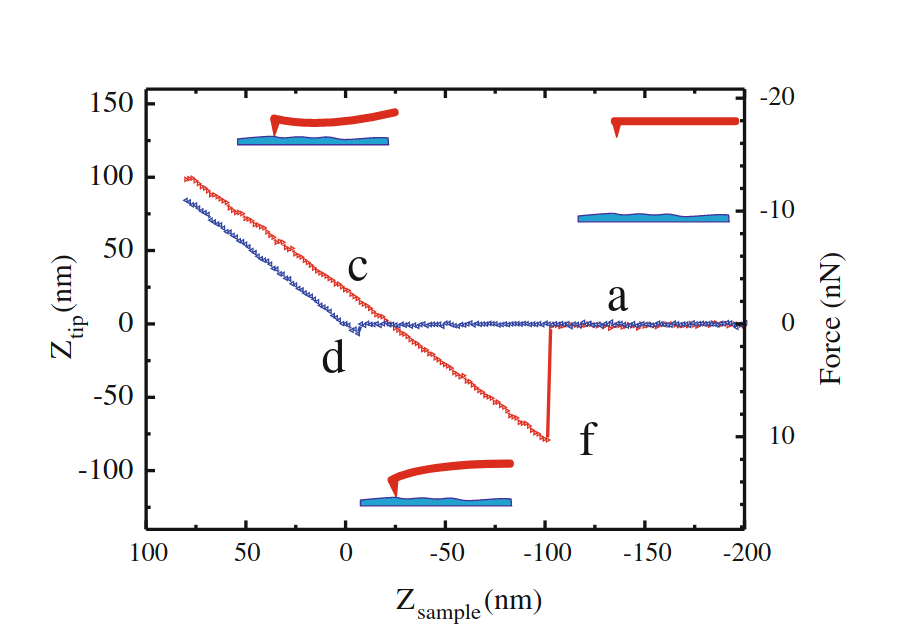
\includegraphics[width = 0.6\textwidth]{pictures/hysterese.png}
            \caption{Abbildung einer Kraft-Distanz-Kurve im Bereich links von c) und d) ist der Versatz der Geraden aufgrund der Hystere der Piezoelemente zu erkennen. Entnommen aus \cite{voigtlander_scanning_2015}}
            \label{fig:hysterese}
          \end{figure}
        
          \FloatBarrier


        \subsection{Disc-Speichermedien}
          Um auf Discs Informationen zu speichern und diese optisch auszulesen, werden entlang von Rillen Absenkungen vorbestimmter Höhe in die Disc gepresst. Wenn ein Ausleselaser über die Rille scannt, kommt
          es an den Kanten der Absenkungen zu destruktiver Interferenz. Der Abfall der reflektierten Intesität wird vom Computer als 1 gespeichert, währen die vorhandene Intensität als 0 gedeutet wird. Da die
          Abfrage in einem vordefinierten Abstand wiederholt wird können so mehrere Einsen sowie Nullen und somit Informationen gespeichert werden. Umso dichter die Rillen aneinandern liegen und je kürzer die
          Länge der Absenkungen ist, desto mehr Informationen können auf den Discs immer gleichen Durchmessers gespeichert werden.



           

